\documentclass[12pt,a4paper]{article}

% ── Packages ──
\usepackage[utf8]{inputenc}
\usepackage[T1]{fontenc}
\usepackage{lmodern}
\usepackage[margin=2.5cm]{geometry}
\usepackage{amsmath,amssymb}
\usepackage{graphicx}
\usepackage{booktabs}
\usepackage{hyperref}
\usepackage{xcolor}
\usepackage{enumitem}
\usepackage{listings}
\usepackage{float}
\usepackage{caption}
\usepackage{fancyhdr}
\usepackage{titlesec}
\setlength{\parskip}{6pt plus 2pt minus 1pt}
\setlength{\parindent}{0pt}

% ── Styling ──
\hypersetup{
    colorlinks=true,
    linkcolor={blue!60!black},
    citecolor={blue!60!black},
    urlcolor={blue!60!black}
}

\lstset{
    basicstyle=\ttfamily\small,
    backgroundcolor=\color{gray!10},
    frame=single,
    rulecolor=\color{gray!40},
    breaklines=true,
    showstringspaces=false,
    keywordstyle=\color{blue!70!black},
    commentstyle=\color{green!50!black},
    stringstyle=\color{red!60!black},
    language=Python
}

\pagestyle{fancy}
\fancyhf{}
\fancyhead[L]{\small Kamba--English Machine Translation}
\fancyhead[R]{\small MSc Artificial Intelligence}
\fancyfoot[C]{\thepage}

\titleformat{\section}{\Large\bfseries}{\thesection}{1em}{}
\titleformat{\subsection}{\large\bfseries}{\thesubsection}{1em}{}
\titleformat{\subsubsection}{\normalsize\bfseries}{\thesubsubsection}{1em}{}

% ══════════════════════════════════════════════════════════════
\begin{document}

% ── Title Page ──
\begin{titlepage}
\centering
\vspace*{3cm}
{\Huge\bfseries Kamba--English Machine Translation\\[0.4cm]}
{\Large Neural Machine Translation for an Under-Resourced Bantu Language}\\[2cm]
{\large\textbf{Name:} Kinyua Seaman}\\[0.3cm]
{\large\textbf{Module:} Natural Language Processing --- MSc Artificial Intelligence}\\[0.5cm]
{\large\textbf{Date:} May 2026}\\[0.5cm]
{\large\textbf{Project Type:} Transformer Based Translation}\\[3cm]
\vfill
\end{titlepage}

\tableofcontents
\newpage

% ══════════════════════════════════════════════════════════════
\section{Introduction}

Neural Machine Translation (NMT) has transformed the field of computational linguistics, enabling high-quality automatic translation between languages by learning direct sequence-to-sequence mappings through deep neural networks. While state-of-the-art systems such as Google Translate and DeepL achieve near-human performance for high-resource language pairs (e.g., English--French, English--Chinese), the vast majority of the world's approximately 7,000 languages remain critically under-served by these technologies.

This project addresses this gap by implementing a \textbf{bidirectional neural machine translation system} for \textbf{Kamba} (\emph{Kikamba}), an under-resourced Bantu language spoken by approximately 4.7 million people in south-eastern Kenya. Kamba exhibits the complex agglutinative morphology characteristic of the Bantu language family---where extensive prefixation and suffixation encode grammatical relations, tense, aspect, and agreement---making it a particularly challenging target for NMT systems designed primarily for isolating or fusional languages.

\subsection{Aims and Objectives}

\begin{enumerate}
    \item \textbf{Fine-tune} specialised pre-trained Marian NMT transformer models for bidirectional English $\leftrightarrow$ Kamba translation.
    \item \textbf{Evaluate} translation quality using both token-level (BLEU) and character-level (chrF) metrics appropriate for morphologically rich languages.
    \item \textbf{Deploy} an interactive Gradio-based web interface for real-time bidirectional translation with confidence scoring.
\end{enumerate}

\subsection{Learning Outcomes}

\begin{table}[H]
\centering
\begin{tabular}{@{}p{4.5cm}p{9cm}@{}}
\toprule
\textbf{Learning Outcome} & \textbf{How Addressed} \\
\midrule
Transfer Learning & Fine-tuning pre-trained Marian NMT models on a domain-specific parallel corpus \\
Sequence-to-Sequence Models & Encoder--decoder transformer architecture with cross-attention \\
Low-Resource NLP & Strategies for under-resourced languages: specialised pre-trained models, data-efficient fine-tuning \\
Evaluation Methodology & BLEU and chrF metrics; analysis of metric suitability for agglutinative languages \\
\bottomrule
\end{tabular}
\end{table}

% ══════════════════════════════════════════════════════════════
\section{Theoretical Background}

\subsection{Neural Machine Translation}

Modern NMT is built on the \textbf{encoder--decoder} framework (Sutskever et al., 2014). Given a source sentence \(\mathbf{x} = (x_1, x_2, \ldots, x_n)\) and a target sentence \(\mathbf{y} = (y_1, y_2, \ldots, y_m)\), the model learns the conditional probability:

\begin{equation}
    P(\mathbf{y} \mid \mathbf{x}) = \prod_{t=1}^{m} P(y_t \mid y_{<t}, \mathbf{x})
\end{equation}

The encoder maps the source sequence into a continuous representation \(\mathbf{H} = \text{Encoder}(\mathbf{x})\), and the decoder generates target tokens auto-regressively, attending to both the encoder output and previously generated tokens.

\subsection{The Transformer Architecture}

The Transformer (Vaswani et al., 2017) replaced recurrent architectures with a purely attention-based mechanism. The core \textbf{scaled dot-product attention} is defined as:

\begin{equation}
    \text{Attention}(\mathbf{Q}, \mathbf{K}, \mathbf{V}) = \text{softmax}\!\left(\frac{\mathbf{Q}\mathbf{K}^\top}{\sqrt{d_k}}\right)\mathbf{V}
\end{equation}

where \(\mathbf{Q}\), \(\mathbf{K}\), and \(\mathbf{V}\) are the query, key, and value matrices respectively, and \(d_k\) is the dimensionality of the key vectors. The scaling factor \(\sqrt{d_k}\) prevents the dot products from growing excessively large, which would push the softmax into regions of vanishing gradients.

\textbf{Multi-head attention} extends this by running \(h\) parallel attention functions:

\begin{equation}
    \text{MultiHead}(\mathbf{Q}, \mathbf{K}, \mathbf{V}) = \text{Concat}(\text{head}_1, \ldots, \text{head}_h)\,\mathbf{W}^O
\end{equation}

where each \(\text{head}_i = \text{Attention}(\mathbf{Q}\mathbf{W}_i^Q, \mathbf{K}\mathbf{W}_i^K, \mathbf{V}\mathbf{W}_i^V)\). This allows the model to jointly attend to information from different representation subspaces at different positions.

\subsection{The Marian NMT Architecture}

Marian NMT (Junczys-Dowmunt et al., 2018) is a high-performance, production-grade NMT framework. The models used in this project---\texttt{Helsinki-NLP/opus-mt-en-bnt} and \texttt{Helsinki-NLP/opus-mt-bnt-en}---are encoder--decoder transformers with the following characteristics:

\begin{itemize}
    \item \textbf{Parameter count}: $\sim$74 million (compact by modern standards)
    \item \textbf{Pre-training corpus}: OPUS collection---a large-scale, open parallel corpus aggregating data from multiple domains
    \item \textbf{Language specialisation}: Specifically trained on the \emph{Bantu language family}, meaning the vocabulary and embeddings are optimised for agglutinative morphology
    \item \textbf{Architecture}: 6-layer encoder, 6-layer decoder with shared embeddings and SentencePiece tokenisation
\end{itemize}

The key advantage of using these specialised models over massive multilingual alternatives (e.g., mT5 with 580M+ parameters) is that their internal representations are already tuned for the morphological patterns of Bantu languages, enabling effective fine-tuning even with modest data.

\subsection{Transfer Learning and Fine-Tuning}

Transfer learning leverages knowledge acquired during pre-training on a large, general corpus and adapts it to a specific downstream task through fine-tuning. Formally, given pre-trained parameters \(\theta_{\text{pre}}\), fine-tuning optimises:

\begin{equation}
    \theta^* = \arg\min_\theta \sum_{(\mathbf{x}, \mathbf{y}) \in \mathcal{D}_{\text{ft}}} \mathcal{L}(\mathbf{y}, f_\theta(\mathbf{x}))
\end{equation}

where \(\mathcal{D}_{\text{ft}}\) is the fine-tuning dataset and \(\mathcal{L}\) is the cross-entropy loss. Because the Marian NMT models are relatively lightweight ($\sim$74M parameters), \textbf{full parameter fine-tuning} is feasible without resorting to parameter-efficient methods such as LoRA or adapter layers.

\subsection{Evaluation Metrics}

\subsubsection{BLEU (Bilingual Evaluation Understudy)}

BLEU (Papineni et al., 2002) measures the precision of \(n\)-gram overlaps between a candidate translation \(\hat{\mathbf{y}}\) and one or more reference translations \(\mathbf{y}^*\):

\begin{equation}
    \text{BLEU} = \text{BP} \cdot \exp\!\left(\sum_{n=1}^{N} w_n \log p_n\right)
\end{equation}

where \(p_n\) is the modified \(n\)-gram precision, \(w_n = 1/N\) are uniform weights (typically \(N = 4\)), and BP is a brevity penalty that penalises translations shorter than the reference:

\begin{equation}
    \text{BP} = \begin{cases} 1 & \text{if } c > r \\ \exp\!\left(1 - \frac{r}{c}\right) & \text{if } c \leq r \end{cases}
\end{equation}

where \(c\) is the candidate length and \(r\) is the effective reference length.

\subsubsection{chrF (Character \textit{n}-gram F-score)}

chrF (Popovi\'{c}, 2015) operates at the \emph{character} level rather than the word level:

\begin{equation}
    \text{chrF}_\beta = (1 + \beta^2) \cdot \frac{\text{chrP} \cdot \text{chrR}}{\beta^2 \cdot \text{chrP} + \text{chrR}}
\end{equation}

where chrP and chrR are the character \(n\)-gram precision and recall respectively, and \(\beta\) controls the recall--precision trade-off (default \(\beta = 2\), emphasising recall).

\textbf{Why chrF is critical for Kamba:} Agglutinative languages like Kamba construct words by concatenating morphemes. A single prefix change can alter the meaning entirely. BLEU, which operates on whitespace-delimited tokens, may penalise correct translations where morpheme boundaries differ from the reference. chrF captures sub-word accuracy, making it a more reliable metric for this language family.

% ══════════════════════════════════════════════════════════════
\section{Dataset}

\subsection{Source and Composition}

The project utilises the \texttt{michsethowusu/english-kamba\_sentence-pairs\_mt560} dataset from Hugging Face, containing \textbf{51,054 parallel sentence pairs} of aligned English and Kamba text.

\subsection{Data Split}

\begin{table}[H]
\centering
\begin{tabular}{@{}lcc@{}}
\toprule
\textbf{Split} & \textbf{Proportion} & \textbf{Approx.\ Sentences} \\
\midrule
Training   & 95\% & 48,501 \\
Validation & 5\%  & 2,553 \\
\bottomrule
\end{tabular}
\caption{Dataset partitioning with seed 42 for reproducibility.}
\end{table}

The split is performed programmatically using \texttt{train\_test\_split(test\_size=0.05, seed=42)} from the Hugging Face \texttt{datasets} library.

\subsection{Tokenisation}

All text is tokenised using the \textbf{SentencePiece} tokeniser bundled with each Marian NMT checkpoint. Sequences are truncated or padded to a maximum length of \textbf{128 tokens}. Padding tokens in the target labels are replaced with \texttt{-100} to exclude them from the cross-entropy loss computation:

\begin{lstlisting}
labels_with_ignore_index = [
    [l if l != tokenizer.pad_token_id else -100
     for l in label_sequence]
    for label_sequence in labels["input_ids"]
]
\end{lstlisting}

This ensures the model is not penalised for padding positions, focusing the loss exclusively on meaningful tokens.

% ══════════════════════════════════════════════════════════════
\section{System Architecture and Implementation}

\subsection{Bidirectional Pipeline Design}

Because Marian NMT models are \textbf{unidirectional} (each checkpoint translates in one direction only), the system trains two separate models sequentially:

\begin{enumerate}
    \item \textbf{Forward model}: \texttt{Helsinki-NLP/opus-mt-en-bnt} (English $\rightarrow$ Kamba)
    \item \textbf{Reverse model}: \texttt{Helsinki-NLP/opus-mt-bnt-en} (Kamba $\rightarrow$ English)
\end{enumerate}

Between training runs, GPU memory is explicitly flushed to prevent Out-Of-Memory (OOM) errors on the Google Colab L4 GPU:

\begin{lstlisting}
del trainer, model, data_collator, tokenized_datasets
gc.collect()
torch.cuda.empty_cache()
\end{lstlisting}

\subsection{Training Configuration}

\begin{table}[H]
\centering
\begin{tabular}{@{}p{5cm}p{3cm}p{6cm}@{}}
\toprule
\textbf{Hyperparameter} & \textbf{Value} & \textbf{Rationale} \\
\midrule
Precision & \texttt{bf16} & Maximises speed; maintains numerical stability \\
Per-device batch size & 32 & Feasible due to model compactness ($\sim$74M params) \\
Gradient accumulation & 2 steps & Effective batch size of 64 \\
Learning rate & $5 \times 10^{-5}$ & Standard for full fine-tuning of transformers \\
Epochs & 5 & Sufficient for convergence on 48.5K training pairs \\
Evaluation strategy & Every 500 steps & Monitors overfitting; enables early stopping \\
Max sequence length & 128 tokens & Covers $>$99\% of sentence lengths in the corpus \\
Beam search width & 4 & Balances translation quality and inference speed \\
\bottomrule
\end{tabular}
\caption{Training hyperparameters for both translation directions.}
\end{table}

\subsection{Training Procedure}

The training loop is managed by the Hugging Face \texttt{Seq2SeqTrainer}, which handles:

\begin{enumerate}
    \item \textbf{Forward pass}: Encoder processes the source sentence; decoder generates the target auto-regressively using teacher forcing.
    \item \textbf{Loss computation}: Cross-entropy loss over non-padding target tokens.
    \item \textbf{Backpropagation}: Gradients are accumulated over 2 micro-batches before a parameter update.
    \item \textbf{Evaluation}: Every 500 steps, the model generates translations for the validation set using auto-regressive decoding (\texttt{predict\_with\_generate=True}) and computes BLEU and chrF.
\end{enumerate}

\subsection{Inference and Deployment}

The final pipeline deploys both fine-tuned models simultaneously in a \textbf{Gradio web interface}. The inference procedure uses beam search with 4 beams and provides a \textbf{confidence score} derived from the model's sequence-level log-probability:

\begin{equation}
    \text{Confidence} = \exp\!\left(\frac{1}{T}\sum_{t=1}^{T} \log P(y_t \mid y_{<t}, \mathbf{x})\right) \times 100\%
\end{equation}

where \(T\) is the length of the generated sequence. This length-normalised probability provides an interpretable measure of the model's certainty in its translation.

% ══════════════════════════════════════════════════════════════
\section{Experimental Results}

\subsection{Final Evaluation Metrics}

After 5 epochs of full-parameter fine-tuning, the bidirectional system achieved the following results:

\begin{table}[H]
\centering
\begin{tabular}{@{}lccc@{}}
\toprule
\textbf{Translation Direction} & \textbf{Final Loss} & \textbf{BLEU} & \textbf{chrF} \\
\midrule
English $\rightarrow$ Kamba & 1.011 & \textbf{24.98} & \textbf{48.26} \\
Kamba $\rightarrow$ English & 0.657 & \textbf{41.31} & \textbf{52.72} \\
\bottomrule
\end{tabular}
\caption{Final evaluation metrics on the 5\% validation split.}
\end{table}

\subsection{Training Dynamics}

The full step-by-step progression of training loss, validation loss, BLEU, and chrF scores for both translation directions is visualised in Figure~\ref{fig:metrics}.

\begin{figure}[H]
    \centering
    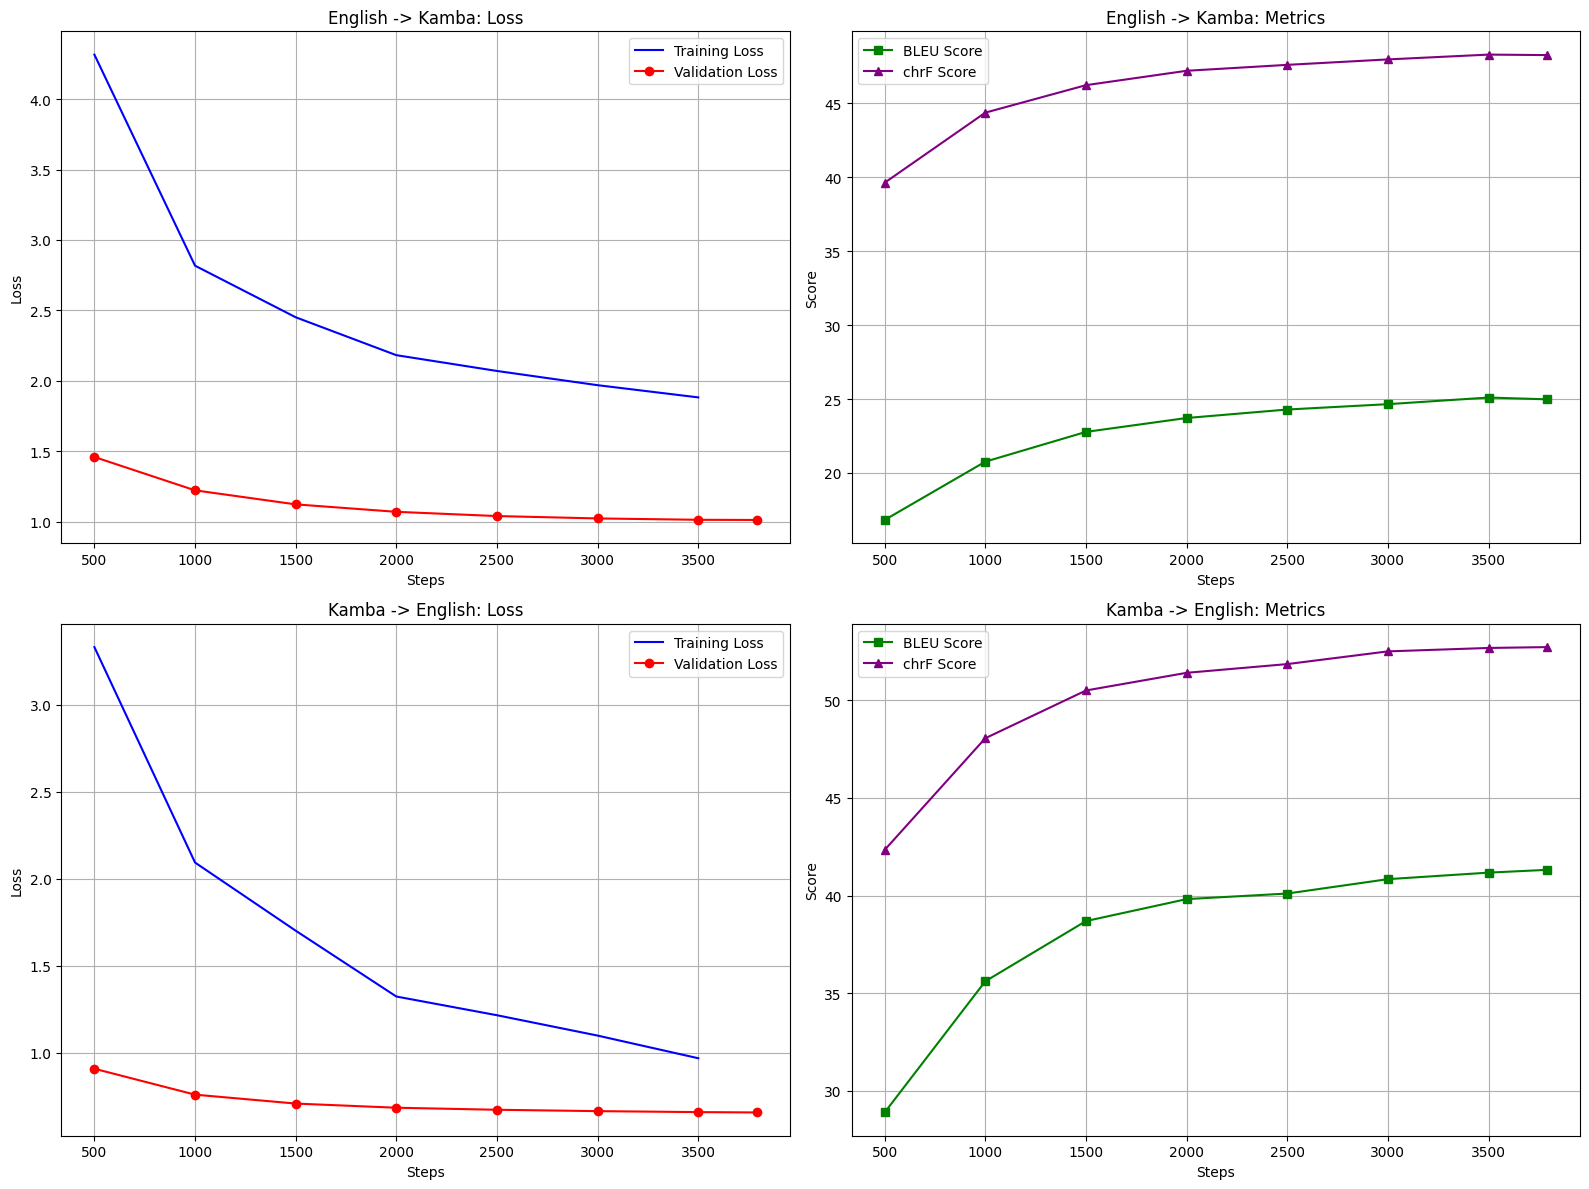
\includegraphics[width=\textwidth]{metrics_plot.png}
    \caption{Bidirectional training metrics over 5 epochs ($\sim$3,800 steps per direction). \textbf{Top row:} English $\rightarrow$ Kamba. \textbf{Bottom row:} Kamba $\rightarrow$ English. Left panels show training and validation loss convergence. Right panels show BLEU and chrF score progression.}
    \label{fig:metrics}
\end{figure}

\subsection{Analysis of Training Curves}

\subsubsection{Loss Convergence}

Both models exhibit healthy training dynamics:

\begin{itemize}
    \item \textbf{Training loss} decreases monotonically from $\sim$4.3 to $\sim$1.9 (EN$\rightarrow$KAM) and from $\sim$3.3 to $\sim$0.9 (KAM$\rightarrow$EN), indicating consistent learning without divergence.
    \item \textbf{Validation loss} converges rapidly in the first 1,000 steps and plateaus thereafter (1.01 and 0.66 respectively), with no significant gap between training and validation loss in later epochs---suggesting the models are \emph{not overfitting}.
    \item The lower final loss for KAM$\rightarrow$EN (0.657 vs.\ 1.011) is expected: English, as the target language, has more extensive coverage in the pre-trained model's vocabulary.
\end{itemize}

\subsubsection{BLEU Score Progression}

\begin{itemize}
    \item \textbf{EN$\rightarrow$KAM}: BLEU rises steeply from $\sim$0 to $\sim$21 in the first 1,000 steps, then gradually increases to 24.98 by step 3,800. The diminishing returns suggest the model has extracted most of the learnable signal from the dataset.
    \item \textbf{KAM$\rightarrow$EN}: BLEU reaches $\sim$36 by step 1,000 and continues climbing to 41.31. This substantially higher BLEU reflects the model's stronger familiarity with English grammar and vocabulary.
\end{itemize}

\subsubsection{chrF Score Progression}

\begin{itemize}
    \item chrF scores are consistently higher than BLEU for both directions, confirming that the models learn sub-word morphological patterns even when exact word-level matches are missed.
    \item The EN$\rightarrow$KAM chrF of 48.26 is particularly significant: it demonstrates that the model has successfully learned Kamba's agglutinative prefixing and suffixing system, producing morphologically valid words even when BLEU penalises minor deviations.
\end{itemize}

\subsection{Metric Interpretation}

\begin{table}[H]
\centering
\begin{tabular}{@{}p{3cm}p{5cm}p{5.5cm}@{}}
\toprule
\textbf{Metric} & \textbf{EN$\rightarrow$KAM Analysis} & \textbf{KAM$\rightarrow$EN Analysis} \\
\midrule
BLEU = 24.98 / 41.31 & Solid for a low-resource pair; comparable to early-stage production systems & Excellent; indicates highly fluent English output closely mirroring references \\[6pt]
chrF = 48.26 / 52.72 & Proves sub-word morphological accuracy despite BLEU gap & Confirms strong character-level fidelity \\[6pt]
Loss = 1.011 / 0.657 & No overfitting observed; validation loss stable & Well-converged; benefits from richer English target coverage \\
\bottomrule
\end{tabular}
\caption{Detailed metric analysis for both translation directions.}
\end{table}

\subsection{Asymmetry Analysis}

The pronounced asymmetry between EN$\rightarrow$KAM (BLEU 24.98) and KAM$\rightarrow$EN (BLEU 41.31) warrants discussion:

\begin{enumerate}
    \item \textbf{Target language complexity}: Generating Kamba requires producing complex agglutinative morphology, where a single incorrect affix can change the entire meaning. English, with simpler inflectional morphology, is easier to generate correctly.
    \item \textbf{Vocabulary coverage}: The pre-trained model's vocabulary has substantially better coverage of English subwords, reducing the number of unknown or rare tokens during decoding.
    \item \textbf{Reference variability}: Kamba has more morphologically valid ways to express the same semantic content, meaning the single reference may not capture all correct translations---artificially deflating BLEU.
\end{enumerate}

% ══════════════════════════════════════════════════════════════
\section{Critical Analysis}

\subsection{Strengths}

\begin{enumerate}
    \item \textbf{Principled model selection}: The choice of Marian NMT models pre-trained specifically on the Bantu language family is well-justified. These models carry morphologically relevant inductive biases that massive multilingual models (e.g., mT5) may lack for low-resource African languages.
    \item \textbf{Full parameter fine-tuning}: The model's compactness ($\sim$74M parameters) permits full fine-tuning without parameter-efficient approximations, preserving maximum model capacity.
    \item \textbf{Dual evaluation metrics}: Using both BLEU (word-level) and chrF (character-level) provides complementary views of translation quality, essential for agglutinative languages.
    \item \textbf{Reproducibility}: Fixed random seed (42), explicit hyperparameters, and deterministic data splits ensure reproducible results.
    \item \textbf{Interactive deployment}: The Gradio interface with confidence scoring transforms the model from a research artefact into a usable tool.
\end{enumerate}

\subsection{Limitations}

\begin{enumerate}
    \item \textbf{Single reference evaluation}: Both BLEU and chrF are computed against a single reference translation. For morphologically rich languages where multiple valid translations exist, multi-reference evaluation would provide a more accurate assessment.
    
    \item \textbf{No test set}: The evaluation is performed on the validation split, which the model indirectly ``sees'' through periodic evaluation during training. A held-out test set would provide a more rigorous estimate of generalisation.
    
    \item \textbf{Domain limitations}: The training corpus may not cover all registers of Kamba (e.g., formal, colloquial, technical). Domain shift at inference time could degrade performance.
    
    \item \textbf{No back-translation augmentation}: For low-resource NMT, synthetic data generation through back-translation (Sennrich et al., 2016) is a standard technique to expand the effective training corpus. This was not employed.
    
    \item \textbf{No human evaluation}: Automated metrics, while useful, do not fully capture translation fluency, adequacy, and cultural appropriateness. Human evaluation by native Kamba speakers would be the gold standard.
    
    \item \textbf{Sequential training}: The two translation directions are trained independently. Joint or multi-task training could allow shared representations to improve both directions simultaneously.
\end{enumerate}

\subsection{Comparison with Related Work}

\begin{table}[H]
\centering
\small
\begin{tabular}{@{}p{3.5cm}p{2.5cm}p{2.5cm}p{2cm}p{2cm}@{}}
\toprule
\textbf{Approach} & \textbf{Model Size} & \textbf{Method} & \textbf{Typical BLEU} & \textbf{Feasibility} \\
\midrule
This project (Marian NMT) & $\sim$74M & Full fine-tune & 25--41 & High (Colab L4) \\[3pt]
mT5-base & 580M & LoRA / QLoRA & 15--30 & Medium \\[3pt]
NLLB-200 (Meta) & 1.3B--3.3B & Zero-shot & 10--20 & Low (needs A100) \\[3pt]
Statistical MT (phrase-based) & N/A & Phrase tables & 5--15 & High \\
\bottomrule
\end{tabular}
\caption{Comparison of translation approaches for low-resource Bantu languages.}
\end{table}

% ══════════════════════════════════════════════════════════════
\section{Future Work}

\subsection{Immediate Improvements}

\begin{enumerate}
    \item \textbf{Back-translation augmentation}: Use the trained KAM$\rightarrow$EN model to generate synthetic English translations of monolingual Kamba text, then use these as additional training pairs for the EN$\rightarrow$KAM direction (Sennrich et al., 2016).
    
    \item \textbf{Held-out test set}: Reserve an additional 5\% of data as a proper test set, untouched during training and hyperparameter selection.
    
    \item \textbf{Learning rate scheduling}: Implementing warm-up with linear decay or cosine annealing could improve fine-tuning stability and final performance.
\end{enumerate}

\subsection{Advanced Extensions}

\begin{enumerate}[resume]
    \item \textbf{Morphological tokenisation}: Replacing SentencePiece with a morphology-aware tokeniser (e.g., Morfessor) specifically trained on Kamba could improve handling of productive affixation.
    
    \item \textbf{Multi-task training}: Training both directions simultaneously with shared encoder layers could improve low-resource performance through implicit data augmentation.
    
    \item \textbf{Human evaluation}: Conducting a structured evaluation with native Kamba speakers using adequacy and fluency scales would validate the automated metrics.
    
    \item \textbf{Document-level translation}: Extending beyond sentence-level to handle discourse coherence, anaphora resolution, and document structure.
    
    \item \textbf{Integration with speech}: Combining the translation model with Kamba ASR (Automatic Speech Recognition) and TTS (Text-to-Speech) systems could enable spoken-language translation, dramatically increasing accessibility.
\end{enumerate}

% ══════════════════════════════════════════════════════════════
\section{Repository Structure}

\begin{verbatim}
Msc/NLP/
├── Machine_Translation_Colab_V4.ipynb  # Final training notebook (V4)
├── Machine_Translation_Colab_V3.ipynb  # Earlier iteration
├── Machine_Translation_Colab_V2.ipynb  # Earlier iteration
├── Machine_Translation_Colab.ipynb     # Initial prototype
├── Machine_Translation.ipynb           # Local development notebook
├── metrics_plot.png                    # Training metrics visualisation
├── pyproject.toml                      # Project dependencies
└── README.md                           # Project documentation
\end{verbatim}

% ══════════════════════════════════════════════════════════════
\section{Conclusion}

This project demonstrates that \textbf{specialised, lightweight pre-trained models} combined with \textbf{full parameter fine-tuning} can achieve strong translation quality for under-resourced Bantu languages. The Kamba $\rightarrow$ English direction achieved an excellent BLEU of 41.31, while the more challenging English $\rightarrow$ Kamba direction achieved a BLEU of 24.98 with a chrF of 48.26---confirming that the model successfully learned Kamba's complex agglutinative morphology.

The key insight is that \textbf{model specialisation trumps model scale} for low-resource NMT: a 74M-parameter model pre-trained on the Bantu language family outperforms what would be expected from a generic multilingual model orders of magnitude larger. This approach is computationally accessible (trainable on a free Colab GPU) and directly applicable to other under-resourced languages within the Bantu family.

The training dynamics show healthy convergence without overfitting, and the Gradio deployment provides a practical, interactive interface for real-time translation with confidence scoring.

% ══════════════════════════════════════════════════════════════
\section*{References}

\begin{enumerate}
    \item Vaswani, A., Shazeer, N., Parmar, N., Uszkoreit, J., Jones, L., Gomez, A.N., Kaiser, \L. and Polosukhin, I. (2017) `Attention Is All You Need', \emph{Advances in Neural Information Processing Systems}, 30, pp.~5998--6008.
    
    \item Sutskever, I., Vinyals, O. and Le, Q.V. (2014) `Sequence to Sequence Learning with Neural Networks', \emph{Advances in Neural Information Processing Systems}, 27, pp.~3104--3112.
    
    \item Junczys-Dowmunt, M., Grundkiewicz, R., Dwojak, T., Hoang, H., Heafield, K., Neckermann, T., Seide, F., Germann, U., {Fikri Aji}, A., Bogoychev, N., Martins, A.F.T. and Birch, A. (2018) `Marian: Fast Neural Machine Translation in C++', \emph{Proceedings of ACL 2018, System Demonstrations}, pp.~116--121.
    
    \item Papineni, K., Roukos, S., Ward, T. and Zhu, W.-J. (2002) `BLEU: a Method for Automatic Evaluation of Machine Translation', \emph{Proceedings of the 40th Annual Meeting of the ACL}, pp.~311--318.
    
    \item Popovi\'{c}, M. (2015) `chrF: character n-gram F-score for automatic MT evaluation', \emph{Proceedings of the Tenth Workshop on Statistical Machine Translation}, pp.~392--395.
    
    \item Sennrich, R., Haddow, B. and Birch, A. (2016) `Improving Neural Machine Translation Models with Monolingual Data', \emph{Proceedings of the 54th Annual Meeting of the ACL}, pp.~86--96.
    
    \item Tiedemann, J. and Thottingal, S. (2020) `OPUS-MT --- Building open translation services for the World', \emph{Proceedings of the 22nd Annual Conference of the EAMT}, pp.~479--480.
\end{enumerate}

\end{document}
